\RequirePackage{amsthm}% sn-jnl defines its theorem styles only if amsthm is loaded first
\documentclass[pdflatex,sn-mathphys,Numbered]{sn-jnl}

\usepackage{graphicx}
\usepackage{multirow}
\usepackage{amsmath,amssymb,amsfonts}
\usepackage{xcolor}
\usepackage{booktabs}
\usepackage{algorithm}
\usepackage{algorithmicx}
\usepackage[noend]{algpseudocode}
\usepackage{url}
\usepackage{longtable}
\usepackage{manyfoot}
\usepackage[title]{appendix}
\usepackage{textcomp}
\usepackage{tabularx}
\usepackage{array}
\usepackage{tikz}

\theoremstyle{thmstyleone}
\newtheorem{theorem}{Theorem}
\newtheorem{lemma}[theorem]{Lemma}
\newtheorem{proposition}[theorem]{Proposition}
\newtheorem{corollary}[theorem]{Corollary}
\theoremstyle{thmstyletwo}
\newtheorem{example}{Example}
\newtheorem{remark}{Remark}
\theoremstyle{thmstylethree}
\newtheorem{definition}{Definition}

\newcommand{\supp}{\operatorname{supp}}
\newcommand{\occ}{\operatorname{occ}}
\newcommand{\ubo}{\operatorname{UBO}}
\newcommand{\cl}{\operatorname{cl}}
\newcommand{\HOI}{\mathcal{H}}
\newcommand{\MHOI}{\mathcal{M}}
\newcommand{\FI}{\mathcal{F}}
\newcommand{\FCI}{\mathcal{C}}
\newcommand{\MFI}{\mathrm{MFI}}
\newcommand{\Max}{\operatorname{Max}}
\newcommand{\capa}{\operatorname{cap}}
\newcommand{\Algo}{MHOI-Miner}

% Generated by make_results.py -- do not edit by hand.
\newcommand{\AblNodesClosedMax}{1.00}
\newcommand{\AblNodesClosedMin}{0.21}
\newcommand{\AblNodesNoHutMax}{1.69}
\newcommand{\AblNodesNoHutMin}{1.00}
\newcommand{\AblNodesNoPreMax}{19.3}
\newcommand{\AblNodesNoPreMin}{3.37}
\newcommand{\AblNodesNoSubMax}{1.01}
\newcommand{\AblNodesNoSubMin}{1.00}
\newcommand{\AblNodesUboMax}{20,999}
\newcommand{\AblNodesUboMin}{5.48}
\newcommand{\AblNodesUboOverB}{1.26--1,088}
\newcommand{\AblNodesWMax}{45.4}
\newcommand{\AblNodesWMin}{3.90}
\newcommand{\AblNodesWOverB}{1.03--2.35}
\newcommand{\AblTimeClosedMax}{2.40}
\newcommand{\AblTimeClosedMin}{1.11}
\newcommand{\AblTimeNoHutMax}{1.04}
\newcommand{\AblTimeNoHutMin}{0.98}
\newcommand{\AblTimeNoPreMax}{3.02}
\newcommand{\AblTimeNoPreMin}{1.29}
\newcommand{\AblTimeNoSubMax}{1.01}
\newcommand{\AblTimeNoSubMin}{0.98}
\newcommand{\AblTimeUboMax}{13.3}
\newcommand{\AblTimeUboMin}{1.37}
\newcommand{\AblTimeWMax}{3.39}
\newcommand{\AblTimeWMin}{1.32}
\newcommand{\FailedDfhoi}{2}
\newcommand{\FailedFull}{0}
\newcommand{\FailedHep}{4}
\newcommand{\FasterCountDfhoi}{19}
\newcommand{\FasterCountHep}{16}
\newcommand{\FasterEtoECountDfhoi}{19}
\newcommand{\FasterEtoECountHep}{16}
\newcommand{\GeoTimeRatioDfhoi}{14.3}
\newcommand{\GeoTimeRatioHep}{8.77}
\newcommand{\MaxClosureEvalRatio}{0.46}
\newcommand{\MaxEtoESlowdownDfhoi}{2.0}
\newcommand{\MaxEtoESlowdownHep}{2.2}
\newcommand{\MaxHoiMhoiKosarak}{4.88}
\newcommand{\MaxHoiMhoiMushroom}{3,134}
\newcommand{\MaxHoiMhoiRetail}{3.93}
\newcommand{\MaxHoiMhoiTten}{27.1}
\newcommand{\MaxNodeReductionDfhoi}{5,837}
\newcommand{\MaxNodeReductionHep}{2,081}
\newcommand{\MaxSlowdownDfhoi}{2.3}
\newcommand{\MaxSlowdownHep}{2.8}
\newcommand{\MaxTimeRatioDfhoi}{882}
\newcommand{\MaxTimeRatioHep}{244}
\newcommand{\MedianEtoERatioDfhoi}{17.9}
\newcommand{\MedianEtoERatioHep}{10.9}
\newcommand{\MedianHoiMhoiRatio}{10.2}
\newcommand{\MedianMemRatioDfhoi}{0.69}
\newcommand{\MedianMemRatioHep}{1.00}
\newcommand{\MedianNodeReductionDfhoi}{125}
\newcommand{\MedianNodeReductionHep}{60.6}
\newcommand{\MedianTimeRatioDfhoi}{24.2}
\newcommand{\MedianTimeRatioHep}{14.9}
\newcommand{\MinHoiMhoiKosarak}{3.94}
\newcommand{\MinHoiMhoiMushroom}{15.5}
\newcommand{\MinHoiMhoiRetail}{3.74}
\newcommand{\MinHoiMhoiTten}{17.1}
\newcommand{\MinNodeReductionDfhoi}{2.57}
\newcommand{\MinNodeReductionHep}{1.92}
\newcommand{\MinTimeRatioDfhoi}{0.43}
\newcommand{\MinTimeRatioHep}{0.36}
\newcommand{\NumDatasets}{five}
\newcommand{\NumOracleCases}{8,100}
\newcommand{\NumOracleDatabases}{900}
\newcommand{\NumSettings}{25}
\newcommand{\OracleMismatches}{0}
\newcommand{\PairCountDfhoi}{23}
\newcommand{\PairCountHep}{21}
\newcommand{\ParityChecked}{23}
\newcommand{\ParityMismatches}{0}
\newcommand{\SetParityChecked}{23}
\newcommand{\SetParityIdentical}{23}

% Generated by case_study/analyze.py -- do not edit by hand.
\newcommand{\CsTransactions}{20,538}
\newcommand{\CsItems}{3,926}
\newcommand{\CsAvgLen}{25.2}
\newcommand{\CsMedLen}{15}
\newcommand{\CsMaxLen}{1,108}
\newcommand{\CsXiRel}{0.2\%}
\newcommand{\CsXiAbs}{41.08}
\newcommand{\CsSigma}{42}
\newcommand{\CsNumHOI}{66}
\newcommand{\CsNumMHOI}{44}
\newcommand{\CsNumMFI}{888,052}
\newcommand{\CsMHOIinMFI}{0}
\newcommand{\CsMHOISingle}{33}
\newcommand{\CsMHOIMulti}{11}
\newcommand{\CsMHOIMaxSize}{4}
\newcommand{\CsMFIisHOI}{0}
\newcommand{\CsMHOIMedSize}{1}
\newcommand{\CsMFIMedSize}{5}
\newcommand{\CsMHOIMedSupp}{916}
\newcommand{\CsMFIMedSupp}{43}
\newcommand{\CsMHOIMedOcc}{48.0}
\newcommand{\CsMFIMedOcc}{0.6}
\newcommand{\CsMHOIMedLen}{34}
\newcommand{\CsMFIMedLen}{508}

\makeatletter\newcommand{\inputrows}[1]{\@@input #1 }\makeatother

\raggedbottom

\begin{document}

\title[Maximal high occupancy itemsets]{Mining maximal high occupancy itemsets with a size-coupled upper bound}

\author*[1]{\fnm{Quan} \sur{Van}}\email{vanhaminhquan2406@gmail.com}
\affil*[1]{\orgname{Independent Researcher}, \orgaddress{\city{Ho Chi Minh City}, \country{Vietnam}}}

\abstract{Occupancy, as defined by Deng, measures how much of its supporting transactions an itemset covers: it is the sum, over these transactions, of the fraction of each transaction that the itemset contains. An itemset is a high occupancy itemset (HOI) if its occupancy reaches a threshold $\xi$. Since the HOIs can be numerous, we study the maximal HOIs (MHOIs), the HOIs with no HOI as a proper superset. We prove that every HOI has support at least $\lceil \xi \rceil$ and every MHOI is closed; that a maximal frequent itemset that is an HOI is an MHOI, whereas an MHOI need not be one; and we observe that, when all transactions have the same length, the upper bound used in existing HOI mining equals the support. We propose an upper bound on the occupancy of the descendants of a search node that fixes the number of added items across the supporting transactions, and prove that it never exceeds the existing bound. The algorithm \Algo{} searches the set-enumeration tree of the frequent itemsets and prunes with this bound, head-union-tail look-ahead and subsumption. Its output agrees with an exact oracle on \NumOracleCases{} randomized cases. On five of the six datasets used by Deng, with his thresholds, it returns the same MHOIs as the two published HOI miners followed by maximality filtering, evaluates a median of \MedianNodeReductionHep{} and \MedianNodeReductionDfhoi{} times fewer itemsets, is faster in most settings and completes all of them; on one sparse dataset it is slower.}

\keywords{Pattern mining, Occupancy, High occupancy itemsets, Maximal itemsets, Closed itemsets, Upper bounds}

\maketitle

%%%%%%%%%%%%%%%%%%%%%%%%%%%%%%%%%%%%%%%%%%%%%%%%%%%%%%%%%%%%%%%%%%%%%%%%%%%%%%%%
\section{Introduction}\label{sec:intro}

A frequent itemset is a set of items that appears together in at least a given number of transactions \cite{agrawal1993mining}. Support does not say how much of a transaction an itemset accounts for: a pair of products that is frequent because it appears in many large orders describes a small part of each of them. Tang et al.\ introduced occupancy to capture this aspect: the occupancy of an itemset in a transaction is the fraction of the transaction that the itemset covers \cite{tang2012occupancy,zhang2015occupancy}. They combined a support threshold with a threshold on the average occupancy. Deng observed that an appropriate pair of thresholds is hard to choose, and defined the occupancy of an itemset as the \emph{sum} of these fractions over its supporting transactions, which grows both with support and with the fraction covered and is used with a single threshold \cite{deng2020hoi}. An itemset whose occupancy reaches the threshold is a high occupancy itemset (HOI). Deng proposed the level-wise algorithm HEP to mine all HOIs, and Nguyen et al.\ the depth-first algorithm DFHOI \cite{nguyen2023dfhoi}; later work studied variants of the problem \cite{datta2022hoimto,kim2022incremental,tran2025namhep,yildirim2025topk,ngo2026topk,cho2026damped}.

The number of HOIs can be large. Deng reports, for example, 331,704 HOIs on the \texttt{mushroom} dataset at a threshold of 4\% of the number of transactions \cite[Table~3]{deng2020hoi}. As for frequent itemsets \cite{bayardo1998maxminer}, the maximal elements give a smaller answer: a maximal HOI (MHOI) is an HOI with no HOI as a proper superset, and every HOI is a subset of an MHOI. Unlike maximal frequent itemsets, MHOIs do not determine all HOIs, because occupancy is not anti-monotone: a subset of an MHOI need not be an HOI. MHOIs report the largest itemsets that reach the threshold; they are not a lossless representation of the HOIs.

This paper is about computing exactly the set of MHOIs. Two approaches follow directly from existing algorithms. The first mines all HOIs with an existing algorithm \cite{deng2020hoi,nguyen2023dfhoi} and keeps the maximal ones; its cost grows with the number of itemsets that these algorithms enumerate. The second mines the maximal frequent itemsets and keeps those that are HOIs; we show that it is incorrect. The contributions are as follows.
\begin{enumerate}
\item We relate MHOIs to frequent, closed and maximal frequent itemsets (Section~\ref{sec:structure}). Every HOI is frequent at the support threshold $\lceil \xi \rceil$, where $\xi$ is the occupancy threshold (this follows from a result of Deng), and every MHOI is closed. Every maximal frequent itemset that is an HOI is an MHOI, but an MHOI need not be a maximal frequent itemset, also when all transactions have the same length; we give examples. When all transactions have the same length $L$, an itemset $X$ is an HOI if and only if its support is at least $\xi L / |X|$, a length-decreasing support constraint in the sense of Seno and Karypis \cite{seno2005ldsc}.
\item We propose a bound on the occupancy of the descendants of a search node that fixes the number $k$ of added items and sums only over the transactions that contain at least $k$ items of the tail (Theorem~\ref{thm:coupled}). We prove that it never exceeds the bound $\ubo$ of Deng \cite{deng2020hoi}, which is used by the existing HOI miners (Theorem~\ref{thm:dominance}), nor a per-transaction bound of the kind used in high-utility mining (Theorem~\ref{thm:pertrans}). We also note that, when all transactions have the same length, $\ubo$ equals the support and prunes nothing beyond it (Proposition~\ref{prop:ubo-uniform}).
\item We present \Algo{}, a depth-first search of the set-enumeration tree of the itemsets with support at least $\lceil \xi \rceil$ that prunes with the bound, with head-union-tail look-ahead and with subsumption by recorded HOIs, and we prove that it returns exactly the MHOIs (Theorem~\ref{thm:correct}).
\item We compare \Algo{} with the two published HOI miners \cite{deng2020hoi,nguyen2023dfhoi}, each followed by maximality filtering, on the datasets and threshold ranges used by Deng \cite{deng2020hoi}, after verifying all implementations against an exact oracle (Section~\ref{sec:exp}). A case study on retail data compares MHOIs with maximal frequent itemsets (Section~\ref{sec:case}).
\end{enumerate}

Section~\ref{sec:related} reviews related work and Section~\ref{sec:problem} defines the problem; a small example database is used throughout to illustrate the definitions, the bounds and a complete run of the algorithm. Section~\ref{sec:structure} proves the structural properties, Section~\ref{sec:bounds} develops the bound and Section~\ref{sec:algo} the algorithm. Section~\ref{sec:exp} reports the experiments, Section~\ref{sec:case} the case study, Section~\ref{sec:limits} the limitations, and Section~\ref{sec:concl} concludes.

%%%%%%%%%%%%%%%%%%%%%%%%%%%%%%%%%%%%%%%%%%%%%%%%%%%%%%%%%%%%%%%%%%%%%%%%%%%%%%%%
\section{Related work}\label{sec:related}

\paragraph{Frequent, closed and maximal itemsets.}
Apriori \cite{agrawal1994fast}, FP-growth \cite{han2000mining} and Eclat \cite{zaki2000scalable} enumerate frequent itemsets using the anti-monotonicity of support. Closed itemsets, which have no proper superset with the same support, form a lossless condensed representation \cite{pasquier1999closed}; CHARM \cite{zaki2002charm} mines them with tidset intersections and LCM \cite{uno2004lcm,uno2005lcm3} with prefix-preserving closure extension, which visits every frequent closed itemset exactly once without storing the itemsets found so far. Maximal frequent itemsets (MFIs) have no frequent proper superset; Max-Miner \cite{bayardo1998maxminer}, MAFIA \cite{burdick2005mafia}, GenMax \cite{gouda2005genmax} and FPMax* \cite{grahne2005fast} mine them with head-union-tail look-ahead and superset checking. Seno and Karypis studied frequent itemsets under a support threshold that decreases with the length of the itemset, and pruned the search with the smallest length that an extension must reach to satisfy the constraint \cite{seno2005ldsc}; on databases whose transactions have equal length, HOIs are itemsets of this kind (Theorem~\ref{thm:mfi}(c)), and the bound of Section~\ref{sec:bounds} expresses a related length argument through the capacities of the transactions. Constraints that are neither anti-monotone nor monotone have been pushed into frequent itemset mining when they are convertible \cite{pei2004convertible}, and combined with closed itemset mining \cite{bonchi2004closedconstrained}; that framework assumes constraints defined by values attached to items, whereas the occupancy of an itemset depends on its supporting transactions. Surveys are available in \cite{aggarwal2014frequent,luna2019review}.

\paragraph{Occupancy.}
Tang et al.\ \cite{tang2012occupancy} and Zhang et al.\ \cite{zhang2015occupancy} defined the average occupancy of an itemset and mined the itemsets that satisfy both a support threshold and an average-occupancy threshold. Deng \cite{deng2020hoi} defined occupancy as the sum of the per-transaction fractions, introduced HOI mining with a single threshold, proved that the occupancy of an itemset is at most its support, and proposed HEP. HEP stores, for each itemset, the list of its supporting transactions with their lengths, generates candidates level by level, and prunes with an upper bound $\ubo$ on the occupancy of all supersets of an itemset (Definition~\ref{def:ubo}). DFHOI \cite{nguyen2023dfhoi} uses the same bound in a depth-first search over equivalence classes. Later work considered transaction occupancy \cite{datta2022hoimto}, incremental databases \cite{kim2022incremental}, an adaptive threshold \cite{tran2025namhep}, top-$k$ mining \cite{yildirim2025topk,ngo2026topk} and data streams \cite{cho2026damped}. These algorithms report all HOIs; we know of no algorithm that mines maximal HOIs.

\paragraph{Utility occupancy.}
Utility occupancy replaces the number of items by their utility \cite{shen2016ocean,gan2020huopm}. Like the occupancy of Tang et al., it is averaged over the supporting transactions and used together with a support threshold. Closed and maximal frequent high-utility occupancy itemsets were studied by Duong et al.\ \cite{duong2024concise} and Hoang et al.\ \cite{hoang2025maxfhuoi}. Their problem has two thresholds and an averaged measure; it does not contain the problem of this paper, whose measure is a sum used with one threshold.

\paragraph{Bounds evaluated before projection.}
Upper bounds on what can still be added in a depth-first enumeration are standard in high-utility itemset mining \cite{liu2012huiminer,zida2017efim,gan2021survey}; EFIM \cite{zida2017efim} computes bounds for the children of a node before projecting their databases. Corollary~\ref{cor:child} applies the same idea to the bound of Theorem~\ref{thm:coupled}.

%%%%%%%%%%%%%%%%%%%%%%%%%%%%%%%%%%%%%%%%%%%%%%%%%%%%%%%%%%%%%%%%%%%%%%%%%%%%%%%%
\section{Problem definition}\label{sec:problem}

Let $I$ be a finite set of items and $D = \langle T_1, \dots, T_n \rangle$ a database of non-empty transactions $T_q \subseteq I$; $|T_q|$ denotes the number of items of $T_q$. For an itemset $X \subseteq I$, $\Gamma(X) = \{ q : X \subseteq T_q \}$ is its cover and $\supp(X) = |\Gamma(X)|$ its support.

\begin{definition}[Occupancy {\cite{deng2020hoi}}]\label{def:occ}
The occupancy of a non-empty itemset $X$ is
\begin{equation}\label{eq:occ}
\occ(X) = \sum_{q \in \Gamma(X)} \frac{|X|}{|T_q|} = |X| \sum_{q \in \Gamma(X)} \frac{1}{|T_q|}.
\end{equation}
\end{definition}

\begin{definition}[HOI and MHOI]\label{def:mhoi}
Let $\xi > 0$ be an occupancy threshold. A non-empty itemset $X$ is a high occupancy itemset (HOI) if $\occ(X) \ge \xi$; $\HOI$ denotes the set of HOIs. An HOI is maximal (an MHOI) if no proper superset of it is an HOI; $\MHOI = \Max(\HOI)$ denotes the set of MHOIs, where $\Max(\mathcal{S})$ is the set of elements of $\mathcal{S}$ with no proper superset in $\mathcal{S}$. The problem is to compute $\MHOI$.
\end{definition}

As in \cite{deng2020hoi}, a threshold can be given relative to the number of transactions: a relative threshold $r$ corresponds to $\xi = r n$. Since $\HOI$ is finite, every HOI is a subset of an MHOI. For a support threshold $\sigma$, $\FI_\sigma$ denotes the set of non-empty itemsets with $\supp(X) \ge \sigma$ and $\MFI_\sigma = \Max(\FI_\sigma)$.

Throughout the paper we illustrate the definitions, the bounds and the algorithm on the database of Table~\ref{tab:example}, with $\xi = 2$.

\begin{table}[t]
\caption{Example database $D$.}\label{tab:example}
\centering
\footnotesize
\begin{tabular}{@{}ccl@{}}
\toprule
TID & Length & Items \\
\midrule
$T_1$ & 3 & $b, d, e$ \\
$T_2$ & 5 & $b, c, d, e, f$ \\
$T_3$ & 4 & $a, c, d, f$ \\
$T_4$ & 2 & $a, f$ \\
$T_5$ & 5 & $a, c, d, e, f$ \\
$T_6$ & 6 & $a, b, c, d, e, f$ \\
$T_7$ & 5 & $a, b, c, d, e$ \\
$T_8$ & 3 & $c, e, f$ \\
\botrule
\end{tabular}
\end{table}

\begin{example}\label{ex:running}
In Table~\ref{tab:example}, $\Gamma(\{a,f\}) = \{3, 4, 5, 6\}$, so
\[
\occ(\{a,f\}) = \frac24 + \frac22 + \frac25 + \frac26 = \frac{67}{30} \approx 2.233,
\]
and $\occ(\{a\}) = \frac14 + \frac12 + \frac15 + \frac16 + \frac15 = \frac{79}{60} \approx 1.317$. With $\xi = 2$, no single item is an HOI, and there are 14 HOIs (Table~\ref{tab:hois}). Four of them have no HOI as a proper superset, so $\MHOI = \{\{a,c,d,e\}, \{a,c,d,f\}, \{b,c,d,e\}, \{c,d,e,f\}\}$. Occupancy is not anti-monotone: $\{c,d,f\}$ is an HOI, with occupancy $49/20 = 2.45$, whereas its subset $\{d,f\}$, with $\Gamma(\{d,f\}) = \{2, 3, 5, 6\}$, has occupancy $2 \left( \frac15 + \frac14 + \frac15 + \frac16 \right) = \frac{49}{30} \approx 1.633$ and is not.
\end{example}

\begin{table}[t]
\caption{The HOIs of the database of Table~\ref{tab:example} with $\xi = 2$, and its maximal frequent itemsets at $\sigma = \lceil \xi \rceil = 2$.}\label{tab:hois}
\centering
\footnotesize
\begin{tabular}{@{}lcccc@{}}
\toprule
Itemset & Cover & Support & $\occ$ & MHOI \\
\midrule
\multicolumn{5}{@{}l}{\emph{HOIs}} \\
$\{a,f\}$ & 3, 4, 5, 6 & 4 & $67/30 \approx 2.233$ & \\
$\{c,d\}$ & 2, 3, 5, 6, 7 & 5 & $61/30 \approx 2.033$ & \\
$\{c,e\}$ & 2, 5, 6, 7, 8 & 5 & $11/5 = 2.2$ & \\
$\{c,f\}$ & 2, 3, 5, 6, 8 & 5 & $23/10 = 2.3$ & \\
$\{d,e\}$ & 1, 2, 5, 6, 7 & 5 & $11/5 = 2.2$ & \\
$\{a,c,d\}$ & 3, 5, 6, 7 & 4 & $49/20 = 2.45$ & \\
$\{b,d,e\}$ & 1, 2, 6, 7 & 4 & $27/10 = 2.7$ & \\
$\{c,d,e\}$ & 2, 5, 6, 7 & 4 & $23/10 = 2.3$ & \\
$\{c,d,f\}$ & 2, 3, 5, 6 & 4 & $49/20 = 2.45$ & \\
$\{c,e,f\}$ & 2, 5, 6, 8 & 4 & $27/10 = 2.7$ & \\
$\{a,c,d,e\}$ & 5, 6, 7 & 3 & $34/15 \approx 2.267$ & yes \\
$\{a,c,d,f\}$ & 3, 5, 6 & 3 & $37/15 \approx 2.467$ & yes \\
$\{b,c,d,e\}$ & 2, 6, 7 & 3 & $34/15 \approx 2.267$ & yes \\
$\{c,d,e,f\}$ & 2, 5, 6 & 3 & $34/15 \approx 2.267$ & yes \\
\midrule
\multicolumn{5}{@{}l}{\emph{Maximal frequent itemsets ($\sigma = 2$)}} \\
$\{a,b,c,d,e\}$ & 6, 7 & 2 & $11/6 \approx 1.833$ & \\
$\{a,c,d,e,f\}$ & 5, 6 & 2 & $11/6 \approx 1.833$ & \\
$\{b,c,d,e,f\}$ & 2, 6 & 2 & $11/6 \approx 1.833$ & \\
\botrule
\end{tabular}
\end{table}

A straightforward way to compute $\MHOI$ is to mine all HOIs with an existing algorithm \cite{deng2020hoi,nguyen2023dfhoi} and to discard every HOI that is a subset of another one. In Example~\ref{ex:running} this computes the 14 HOIs and discards 10 of them. Its cost is that of enumerating all HOIs, together with all itemsets that the HOI miner examines to find them, and of comparing the HOIs with each other, although most of them are discarded. Section~\ref{sec:results} shows that on the benchmark datasets the HOIs outnumber the MHOIs by a median factor of \MedianHoiMhoiRatio{} and by up to \MaxHoiMhoiMushroom{}, and that the HOI miners exceed the time or memory limit at thresholds where the MHOIs are few. This motivates a search that is directed at the maximal HOIs and prunes the itemsets that cannot lead to one.

%%%%%%%%%%%%%%%%%%%%%%%%%%%%%%%%%%%%%%%%%%%%%%%%%%%%%%%%%%%%%%%%%%%%%%%%%%%%%%%%
\section{Structural properties}\label{sec:structure}

\begin{lemma}[{\cite[Theorem~1]{deng2020hoi}}]\label{lem:occsupp}
$\occ(X) \le \supp(X)$ for every non-empty itemset $X$. Consequently $\HOI \subseteq \FI_{\sigma}$ with $\sigma = \lceil \xi \rceil$.
\end{lemma}
\begin{proof}
Each term $|X|/|T_q|$ of \eqref{eq:occ} is at most $1$ because $X \subseteq T_q$. If $\occ(X) \ge \xi$, then $\supp(X) \ge \xi$, and $\supp(X) \ge \lceil \xi \rceil$ because support is an integer.
\end{proof}

Throughout, $\sigma = \lceil \xi \rceil$. The closure of an itemset $X$ with $\supp(X) > 0$ is $\cl(X) = \bigcap_{q \in \Gamma(X)} T_q$, and $X$ is closed if $\cl(X) = X$; $X \subseteq \cl(X)$ and $\Gamma(\cl(X)) = \Gamma(X)$ \cite{pasquier1999closed}. Let $\FCI_\sigma$ be the set of closed itemsets in $\FI_\sigma$.

\begin{lemma}\label{lem:closure}
If $\supp(X) > 0$, then $\occ(\cl(X)) = \frac{|\cl(X)|}{|X|} \occ(X) \ge \occ(X)$. In particular, if $X \in \HOI$ then $\cl(X) \in \HOI$.
\end{lemma}
\begin{proof}
$X$ and $\cl(X)$ have the same cover, so the sum in \eqref{eq:occ} is the same for both; only the factor $|X|$ changes, and $|\cl(X)| \ge |X|$.
\end{proof}

\begin{example}\label{ex:closure}
In Table~\ref{tab:example}, $\cl(\{d,f\}) = T_2 \cap T_3 \cap T_5 \cap T_6 = \{c,d,f\}$, and $\occ(\{c,d,f\}) = \frac32 \occ(\{d,f\}) = \frac32 \cdot \frac{49}{30} = \frac{49}{20}$. All 14 HOIs of Table~\ref{tab:hois} are closed.
\end{example}

\begin{theorem}\label{thm:maxclosed}
Every MHOI is closed, and $\MHOI = \Max(\HOI \cap \FCI_\sigma)$.
\end{theorem}
\begin{proof}
Let $X \in \MHOI$. If $X$ were not closed, $\cl(X) \supsetneq X$ would be an HOI by Lemma~\ref{lem:closure}, contradicting maximality. By Lemma~\ref{lem:occsupp}, $X \in \FI_\sigma$, so $X \in \HOI \cap \FCI_\sigma$; since $X$ has no proper superset in $\HOI$, it has none in $\HOI \cap \FCI_\sigma$.
Conversely, let $X \in \Max(\HOI \cap \FCI_\sigma)$ and suppose that some $Y \in \HOI$ satisfies $Y \supsetneq X$. By Lemmas~\ref{lem:closure} and~\ref{lem:occsupp}, $\cl(Y) \in \HOI \cap \FCI_\sigma$ and $\cl(Y) \supseteq Y \supsetneq X$, a contradiction. Hence $X \in \MHOI$.
\end{proof}

Theorem~\ref{thm:maxclosed} restricts the search to frequent closed itemsets. The next result relates MHOIs to maximal frequent itemsets.

\begin{theorem}\label{thm:mfi}
\begin{enumerate}
\item[(a)] $\MFI_\sigma \cap \HOI \subseteq \MHOI$.
\item[(b)] The inclusion $\MHOI \subseteq \MFI_\sigma$ does not hold in general, even when all transactions have the same length.
\item[(c)] If all transactions have length $L$, then $X \in \HOI$ if and only if $\supp(X) \ge \xi L / |X|$.
\end{enumerate}
\end{theorem}
\begin{proof}
(a) Let $M \in \MFI_\sigma \cap \HOI$. A proper superset $Y$ of $M$ that is an HOI would satisfy $\supp(Y) \ge \sigma$ by Lemma~\ref{lem:occsupp}, contradicting $M \in \MFI_\sigma$.
(b) In Example~\ref{ex:running}, $\sigma = 2$ and $\MFI_2 = \{\{a,b,c,d,e\}, \{a,c,d,e,f\}, \{b,c,d,e,f\}\}$, each of occupancy $11/6 < 2$ (Table~\ref{tab:hois}); none of them is an HOI, and none of the four MHOIs is an MFI, so keeping the MFIs that are HOIs returns the empty set. For equal lengths, let $L = 3$, $\xi = 2$ and $D = \langle \{a,b,x_1\}, \{a,b,x_2\}, \{a,c,x_3\}, \{a,c,x_4\}, \{a,d,x_5\}, \{a,d,x_6\} \rangle$. Then $\occ(\{a\}) = 6/3 = 2$; each of $\{a,b\}$, $\{a,c\}$, $\{a,d\}$ has support $2$ and occupancy $4/3$; every other itemset with two or more items has support at most $1$ and occupancy at most $1$; and every item other than $a$ has occupancy at most $2/3$. Hence $\MHOI = \{\{a\}\}$, while $\MFI_2 = \{\{a,b\}, \{a,c\}, \{a,d\}\}$.
(c) With equal lengths, $\occ(X) = |X| \supp(X) / L$.
\end{proof}

By (c), on databases with equal transaction lengths the HOIs are the itemsets that satisfy the length-decreasing support constraint $f(\ell) = \xi L / \ell$ of \cite{seno2005ldsc}, and the MHOIs are the maximal such itemsets. A superset of an HOI is longer, so it needs less support, but it can have much less support; this is why (b) holds also for equal lengths.

%%%%%%%%%%%%%%%%%%%%%%%%%%%%%%%%%%%%%%%%%%%%%%%%%%%%%%%%%%%%%%%%%%%%%%%%%%%%%%%%
\section{Upper bounds}\label{sec:bounds}

\subsection{An existing upper bound}

\begin{definition}[$\ubo$ {\cite[Definition~7]{deng2020hoi}}]\label{def:ubo}
Let $X$ be an itemset with $\supp(X) > 0$, and let $l_1 < \dots < l_u$ be the distinct lengths of the transactions in $\Gamma(X)$. For $1 \le x \le u$, let
\[
\ubo_x(X) = l_x \sum_{q \in \Gamma(X),\, |T_q| \ge l_x} \frac{1}{|T_q|},
\]
and $\ubo(X) = \max_{1 \le x \le u} \ubo_x(X)$.
\end{definition}

Deng proved that $\occ(Y) \le \ubo(X)$ for every superset $Y$ of $X$ \cite[Theorem~4]{deng2020hoi}; the HOI miners of \cite{deng2020hoi,nguyen2023dfhoi} do not extend $X$ when $\ubo(X) < \xi$.

\begin{example}\label{ex:ubo}
The cover of $\{a,c,d,e\}$ in Table~\ref{tab:example} consists of $T_5$, $T_6$ and $T_7$, of lengths $5$, $6$ and $5$. Hence $\ubo_1 = 5 \left( \frac15 + \frac16 + \frac15 \right) = \frac{17}{6}$ and $\ubo_2 = 6 \cdot \frac16 = 1$, so $\ubo(\{a,c,d,e\}) = \frac{17}{6} \approx 2.833 \ge 2$: with $\xi = 2$, $\ubo$ does not prune the supersets of $\{a,c,d,e\}$.
\end{example}

\begin{proposition}\label{prop:ubo-uniform}
If all transactions of $\Gamma(X)$ have the same length, then $\ubo(X) = \supp(X)$. In particular, if all transactions of $D$ have the same length, $\ubo$ prunes no itemset $X$ with $\supp(X) \ge \xi$.
\end{proposition}
\begin{proof}
With a single length $l_1$, $\ubo(X) = \ubo_1(X) = l_1 \cdot \supp(X) / l_1$.
\end{proof}

On such databases, a search that prunes with $\ubo$ enumerates all itemsets with support at least $\sigma$, as the baseline algorithm of \cite{deng2020hoi} does.

\subsection{A size-coupled bound}

Consider a node of a depth-first search that holds an itemset $C$ with $\supp(C) \ge \sigma$, and a set $R$ of items not in $C$, its tail, such that every descendant of the node is an itemset $C \cup Z$ with $\emptyset \ne Z \subseteq R$ (for the search of Section~\ref{sec:algo}, this is Lemma~\ref{lem:desc}). For $q \in \Gamma(C)$, the capacity of transaction $q$ is $\capa(q) = |T_q \cap R|$. For $k \ge 1$, let
\[
Q_k = \{ q \in \Gamma(C) : \capa(q) \ge k \}, \qquad S_k = \sum_{q \in Q_k} \frac{1}{|T_q|}.
\]

\begin{theorem}[Size-coupled bound]\label{thm:coupled}
Let
\begin{equation}\label{eq:coupled}
B(C) = \max \{ (|C| + k) \, S_k : k \ge 1,\ |Q_k| \ge \sigma \},
\end{equation}
with $B(C) = 0$ if no $k$ satisfies $|Q_k| \ge \sigma$. Every itemset $Y = C \cup Z$ with $\emptyset \neq Z \subseteq R$ that is an HOI satisfies $\occ(Y) \le B(C)$. Hence, if $B(C) < \xi$, no descendant of the node is an HOI.
\end{theorem}
\begin{proof}
Let $k = |Z| \ge 1$. Every $q \in \Gamma(Y)$ belongs to $\Gamma(C)$ and contains $Z \subseteq R$, so $\capa(q) \ge k$ and $\Gamma(Y) \subseteq Q_k$. Since $Y$ is an HOI, $|Q_k| \ge \supp(Y) \ge \sigma$ by Lemma~\ref{lem:occsupp}. As $|Y| = |C| + k$ and all terms are positive,
\[
\occ(Y) = (|C| + k) \sum_{q \in \Gamma(Y)} \frac{1}{|T_q|} \le (|C| + k) \, S_k \le B(C).
\]
\end{proof}

\begin{theorem}\label{thm:dominance}
$B(C) \le \ubo(C)$.
\end{theorem}
\begin{proof}
If $B(C) = 0$ there is nothing to prove. Otherwise let $k \ge 1$ attain the maximum in \eqref{eq:coupled}, so $Q_k \neq \emptyset$, and let $l = \min \{ |T_q| : q \in Q_k \}$, which is one of the lengths $l_x$ of Definition~\ref{def:ubo}. For $q \in Q_k$, $C$ and $T_q \cap R$ are disjoint subsets of $T_q$, so $|T_q| \ge |C| + \capa(q) \ge |C| + k$; hence $l \ge |C| + k$. Every $q \in Q_k$ satisfies $|T_q| \ge l$, so
\[
B(C) = (|C| + k) \, S_k \le l \sum_{q \in \Gamma(C),\, |T_q| \ge l} \frac{1}{|T_q|} = \ubo_x(C) \le \ubo(C).
\]
\end{proof}

Bounds based on the items that remain to be added are standard in high-utility itemset mining \cite{liu2012huiminer,zida2017efim,gan2020huopm}. Transferred to occupancy, such a bound lets every transaction assume the largest extension it can hold:
\[
W(C) = \sum_{q \in \Gamma(C),\ \capa(q) \ge 1} \frac{|C| + \capa(q)}{|T_q|}.
\]
Every HOI $Y = C \cup Z$ with $\emptyset \ne Z \subseteq R$ satisfies $\occ(Y) \le W(C)$, since each term of $\occ(Y)$ is at most the corresponding term of $W(C)$.

\begin{theorem}\label{thm:pertrans}
$B(C) \le W(C)$.
\end{theorem}
\begin{proof}
For $k \ge 1$ with $|Q_k| \ge \sigma$, every $q \in Q_k$ satisfies $\capa(q) \ge k \ge 1$, so
$(|C| + k) S_k = \sum_{q \in Q_k} \frac{|C| + k}{|T_q|} \le \sum_{q \in Q_k} \frac{|C| + \capa(q)}{|T_q|} \le W(C)$.
\end{proof}

$W$ lets each transaction assume its own extension size; $B$ uses one size $k$ for all transactions that support the extension. $\ubo$ bounds the size of a superset by the length of the shortest transaction that may contain it. $B$ bounds it by the number of tail items that the transactions actually contain, and uses the same size for all transactions that support the superset.

\begin{example}\label{ex:coupled-running}
In the search of Section~\ref{sec:algo} on Table~\ref{tab:example} (Example~\ref{ex:search}), the node that holds $C = \{a,c,d,e\}$ has the tail $R = \{f\}$. Among the three transactions of $\Gamma(C)$, $T_5$ and $T_6$ contain $f$ and $T_7$ does not, so $Q_1 = \{5, 6\}$, $|Q_1| = 2 \ge \sigma$, and
\[
B(\{a,c,d,e\}) = (4 + 1)\left( \frac15 + \frac16 \right) = \frac{11}{6} \approx 1.833 < 2.
\]
Rule P1 skips the subtree of the node, whereas $\ubo(\{a,c,d,e\}) = 17/6 \ge 2$ (Example~\ref{ex:ubo}); the node itself, an HOI, is recorded. Its only descendant, $\{a,c,d,e,f\}$, has occupancy $11/6$. $\ubo$ allows a superset of $\{a,c,d,e\}$ to be supported by $T_7$, which contains no item of the tail; $B$ counts only the transactions that contain a tail item.
\end{example}

\begin{example}\label{ex:coupled}
Let all transactions have length $L = 10$, $|C| = 1$, $\supp(C) = 10$, $\capa(q) = 1$ for every $q \in \Gamma(C)$, and $\xi = 5$. By Proposition~\ref{prop:ubo-uniform}, $\ubo(C) = 10 \ge \xi$, so $\ubo$ does not prune. $Q_1 = \Gamma(C)$ and $Q_k = \emptyset$ for $k \ge 2$, so $B(C) = 2 \cdot 10/10 = 2 < \xi$ and the node is pruned. Indeed, every descendant has two items and support at most $10$, hence occupancy at most $2$.
\end{example}

If all transactions have length $L$, then $S_k = |Q_k| / L$ and $B(C) = \max \{ (|C| + k) |Q_k| / L : k \ge 1,\ |Q_k| \ge \sigma \}$: the bound is the largest value of $|Y| \cdot \supp / L$ that the capacities allow, in agreement with Theorem~\ref{thm:mfi}(c).

A parent can evaluate the bound for a child before building the child's database. Let the tail $R$ be ordered, let $e \in R$, and let the child node hold $C \cup \{e\}$ with tail $R_{>e} = \{ x \in R : x \succ e \}$. For $q \in \Gamma(C \cup \{e\})$ let $\capa_e(q) = |T_q \cap R_{>e}|$; it is obtained from the transactions of the parent by counting the tail items after $e$.

\begin{corollary}[Child bound]\label{cor:child}
For $k \ge 0$ let $Q^e_k = \{ q \in \Gamma(C \cup \{e\}) : \capa_e(q) \ge k \}$ and $S^e_k = \sum_{q \in Q^e_k} 1/|T_q|$. Every itemset $Y = C \cup \{e\} \cup Z'$ with $Z' \subseteq R_{>e}$ (possibly empty) that is an HOI satisfies
\[
\occ(Y) \le B_e(C) := \max \{ (|C| + 1 + k) \, S^e_k : k \ge 0,\ |Q^e_k| \ge \sigma \},
\]
with $B_e(C) = 0$ if no $k$ satisfies $|Q^e_k| \ge \sigma$.
\end{corollary}
\begin{proof}
Apply the argument of Theorem~\ref{thm:coupled} with $k = |Z'| \ge 0$: every $q \in \Gamma(Y)$ belongs to $\Gamma(C \cup \{e\})$ and contains $Z' \subseteq R_{>e}$.
\end{proof}

\begin{example}\label{ex:child}
In the same search, the node that holds $C = \{b\}$, with $\Gamma(C) = \{1, 2, 6, 7\}$, has the tail $R = (a, c, d, e, f)$ in this order. For the child with $a$: $\Gamma(C \cup \{a\}) = \{6, 7\}$, $R_{>a} = \{c, d, e, f\}$, $\capa_a(6) = 4$ and $\capa_a(7) = 3$. For $k = 0, \dots, 3$ both transactions qualify, and for $k = 4$ only $T_6$ does, which is fewer than $\sigma = 2$. Hence
\[
B_a(C) = \max_{0 \le k \le 3} (2 + k) \left(\frac16 + \frac15\right) = 5 \cdot \frac{11}{30} = \frac{11}{6} \approx 1.833 < 2,
\]
and the child $\{a,b\}$ is skipped with its subtree, which contains 8 itemsets with support at least $2$; the largest occupancy among them is that of $\{a,b,c,d,e\}$, $11/6$. For the child with $f$, $\Gamma(C \cup \{f\}) = \{2, 6\}$ and no tail item follows $f$, so $B_f(C) = 2 \left(\frac15 + \frac16\right) = \frac{11}{15} < 2$.
\end{example}

\paragraph{Computation.}
Given the pairs $(|T_q|, \capa(q))$ of the node, accumulating $1/|T_q|$ and the number of transactions per capacity value and summing them from the largest capacity down to $1$ gives all $S_k$ and $|Q_k|$, and hence $B(C)$, in $O(r + c_{\max})$ time, where $r$ is the number of rows of the node (transactions of the cover, merged as described in Section~\ref{sec:algo}) and $c_{\max}$ the largest capacity.

%%%%%%%%%%%%%%%%%%%%%%%%%%%%%%%%%%%%%%%%%%%%%%%%%%%%%%%%%%%%%%%%%%%%%%%%%%%%%%%%
\section{The \Algo{} algorithm}\label{sec:algo}

\subsection{Search space}

Order the items $i$ with $\supp(\{i\}) \ge \sigma$ by increasing support, breaking ties by a fixed order on item identifiers. \Algo{} searches the set-enumeration tree of the itemsets with support at least $\sigma$ \cite{bayardo1998maxminer}, which contains all HOIs by Lemma~\ref{lem:occsupp}. The root holds the empty itemset. A node holding $C$, whose last item in the order is $\mathrm{last}(C)$ (none at the root), has a child $C \cup \{e\}$ for every item $e$ of its tail
\[
R(C) = \{ e \succ \mathrm{last}(C) : \supp(C \cup \{e\}) \ge \sigma \},
\]
with $\mathrm{last}(C)$ taken to precede every item at the root. Since support is anti-monotone, every itemset with support at least $\sigma$ is the itemset of exactly one node: its items, added in increasing order, form a path from the root.

\begin{lemma}\label{lem:desc}
Every descendant of the node holding $C$ is an itemset $C \cup Z$ with $\emptyset \neq Z \subseteq R(C)$. Moreover, for $e \in R(C)$, the child $C \cup \{e\}$ and all its descendants are contained in $C \cup \{e\} \cup \{ x \in R(C) : x \succ e \}$.
\end{lemma}
\begin{proof}
The tail of the child $C \cup \{e\}$ consists of items $x \succ e$ with $\supp(C \cup \{e, x\}) \ge \sigma$; as $\Gamma(C \cup \{e,x\}) \subseteq \Gamma(C \cup \{x\})$, these items satisfy $\supp(C \cup \{x\}) \ge \sigma$, so $R(C \cup \{e\}) \subseteq \{ x \in R(C) : x \succ e \}$. Both claims follow by induction on the depth.
\end{proof}

Lemma~\ref{lem:desc} is the setting of Section~\ref{sec:bounds}: a node $C$ with a tail $R$ whose descendants are of the form $C \cup Z$, $\emptyset \neq Z \subseteq R$. The search does not restrict itself to closed itemsets, although every MHOI is closed (Theorem~\ref{thm:maxclosed}): a version that enumerates only closed itemsets by prefix-preserving closure extension \cite{uno2004lcm} visits fewer nodes, but computing closures at every node made it slower on all our datasets (Section~\ref{sec:ablation}). Closures are used only by rule P2 below.

\subsection{Conditional databases}

A node keeps the transactions of its cover, projected on the items of its tail. Two projected transactions with the same items \emph{and the same original length} are merged into one row with a weight equal to the number of merged transactions.

\begin{lemma}\label{lem:merge}
Merging rows with the same projected items and the same original length preserves, for every node and every candidate extension, the support, the sum $\sum 1/|T_q|$ over the cover, and the multiset of pairs $(|T_q|, \capa(q))$.
\end{lemma}
\begin{proof}
Each of these quantities is a sum or a multiset over transactions in which a transaction enters only through its projected items and its original length, and the weight counts multiplicity.
\end{proof}

Merging on items alone, as in frequent itemset mining \cite{uno2005lcm3}, would change $\sum 1/|T_q|$ and therefore occupancy.

\subsection{Pruning rules}

At a node holding $C$ with tail $R$, \Algo{} applies the following rules, in this order.
\begin{enumerate}
\item[\textbf{P1}] (subtree bound) If $B(C) < \xi$ (Theorem~\ref{thm:coupled}), no descendant is an HOI; the subtree is skipped.
\item[\textbf{P2}] (head-union-tail) Let $H = C \cup R$. If $\occ(H) \ge \xi$, then $\cl(H)$ is an HOI (Lemma~\ref{lem:closure}) that contains every descendant; it is recorded unless it is a subset of a recorded itemset, and the subtree is skipped. $\cl(H)$ is computed as the intersection of the transactions of $\Gamma(H)$.
\item[\textbf{P3}] (subsumption) If $C \cup R$ is a subset of a recorded itemset, no descendant is an MHOI that has not been recorded; the subtree is skipped.
\item[\textbf{P4}] (child bound) Before generating the child for $e \in R$, if $B_e(C) < \xi$ (Corollary~\ref{cor:child}), the child and its subtree are skipped without building the child's database.
\end{enumerate}
$K$ denotes the set of recorded itemsets. \textsc{Mine} returns true when it has found that some HOI contains $C$: $C$ itself, an HOI recorded by P2 or found below a child, or a recorded HOI that contains $C \cup R$ (P3). A node whose itemset is an HOI is recorded when its tail is empty or P1 applies, and after its children have been explored if none of them returned true; it is not recorded when P2 or P3 applies, since an HOI that contains it is then known. After the search, the recorded itemsets that are subsets of other recorded itemsets are removed. Rule P2 is the head-union-tail look-ahead of maximal frequent itemset mining \cite{bayardo1998maxminer,burdick2005mafia} with the support condition replaced by the occupancy condition, and rule P3 is the corresponding superset check.

\begin{algorithm}[t]
\caption{\Algo}\label{alg:main}
\begin{algorithmic}[1]
\Require database $D$, occupancy threshold $\xi$
\Ensure the set $\MHOI$ of MHOIs
\State $\sigma \gets \lceil \xi \rceil$; $K \gets \emptyset$ \Comment{set of recorded HOIs}
\State build the root database (items with support $\ge \sigma$, merged rows); \Call{Mine}{$\emptyset$, root rows, none}
\State \Return the elements of $K$ that are not subsets of other elements of $K$
\Statex
\Function{Mine}{$C$, rows, last} \Comment{returns true only if some HOI contains $C$}
  \State compute $\occ(C)$, the tail $R$ and the capacities from the rows
  \State $f \gets [C \neq \emptyset \text{ and } \occ(C) \ge \xi]$
  \If{$R = \emptyset$ \textbf{or} $B(C) < \xi$} \Comment{P1}
    \State \textbf{if} $f$ \textbf{then} add $C$ to $K$; \Return $f$
  \EndIf
  \If{$\occ(C \cup R) \ge \xi$} \Comment{P2}
    \State add $\cl(C \cup R)$ to $K$ unless it is a subset of an element of $K$; \Return true
  \EndIf
  \If{$C \cup R \subseteq M$ for some $M \in K$} \Return true \Comment{P3}
  \EndIf
  \State $g \gets$ false
  \For{$e \in R$ in increasing order}
    \If{$B_e(C) < \xi$} \textbf{continue} \Comment{P4}
    \EndIf
    \State build the rows of $C \cup \{e\}$ (projection on the items after $e$ with support $\ge \sigma$ in $\Gamma(C \cup \{e\})$, merging)
    \State \textbf{if} \Call{Mine}{$C \cup \{e\}$, its rows, $e$} \textbf{then} $g \gets$ true
  \EndFor
  \State \textbf{if} $f$ \textbf{and not} $g$ \textbf{then} add $C$ to $K$
  \State \Return $f$ \textbf{or} $g$
\EndFunction
\end{algorithmic}
\end{algorithm}

\subsection{Example}

\begin{example}\label{ex:search}
We run \Algo{} on Table~\ref{tab:example} with $\xi = 2$, so $\sigma = 2$. The supports of $a, b, c, d, e, f$ are $5, 4, 6, 6, 6, 6$, so the items are ordered $b \prec a \prec c \prec d \prec e \prec f$ (ties broken alphabetically). The set-enumeration tree of the itemsets with support at least $2$ has 55 nodes besides the root. Table~\ref{tab:trace} lists the 16 nodes that \Algo{} visits, in the order of the search, and Fig.~\ref{fig:search} shows them together with the parts of the tree that are skipped.

\emph{Root.} Every item is in the tail, so $\capa(q) = |T_q|$ for every transaction and $B(\emptyset) = \max_k k \sum_{|T_q| \ge k} 1/|T_q| = 101/20 = 5.05$, attained at $k = 3$. The child bounds of $e$ and $f$ are $9/5$ and $33/20$, so rule P4 skips $\{e\}$ and $\{f\}$ and their subtrees; the children $\{b\}$, $\{a\}$, $\{c\}$ and $\{d\}$ are built.

\emph{Subtree of $\{b\}$.} P4 skips the extensions of $\{b\}$ with $a$ (Example~\ref{ex:child}), $e$ and $f$. Along $\{b,c\}$ and $\{b,c,d\}$, which are not HOIs, P4 skips four more extensions, and the search reaches $\{b,c,d,e\}$, an HOI whose tail is $\{f\}$ and whose bound is $B = 11/6 < 2$: P1 records it. Similarly, $\{b,d,e\}$, reached through $\{b,d\}$, is an HOI with tail $\{f\}$ and $B = 22/15 < 2$, and P1 records it as well.

\emph{Subtree of $\{a\}$.} Along $\{a,c\}$ the search reaches $\{a,c,d\}$, an HOI with two children: $\{a,c,d,e\}$, recorded by P1 (Example~\ref{ex:coupled-running}), and $\{a,c,d,f\}$, whose tail is empty and which is recorded. At $\{a,d\}$, P4 skips both extensions, so the node has no child. $\{a,e\}$ is skipped by P4, and $\{a,f\}$, an HOI with an empty tail, is recorded.

\emph{Node $\{c\}$.} The tail is $(d, e, f)$, and the transactions that contain all three items are $T_2$, $T_5$ and $T_6$. Hence $\occ(\{c,d,e,f\}) = 4 \left(\frac15 + \frac15 + \frac16\right) = \frac{34}{15} \ge 2$, and rule P2 records $\cl(\{c,d,e,f\}) = T_2 \cap T_5 \cap T_6 = \{c,d,e,f\}$. The seven itemsets of the subtree of $\{c\}$ are not visited; all of them are HOIs and subsets of $\{c,d,e,f\}$.

\emph{Node $\{d\}$.} $C \cup R = \{d,e,f\} \subseteq \{c,d,e,f\}$, which has been recorded, so rule P3 skips the subtree, which contains the HOI $\{d,e\}$.

The search visits 16 of the 56 nodes. It records $\{b,c,d,e\}$, $\{b,d,e\}$, $\{a,c,d,e\}$, $\{a,c,d,f\}$, $\{a,f\}$ and $\{c,d,e,f\}$; the final filter removes $\{b,d,e\} \subset \{b,c,d,e\}$ and $\{a,f\} \subset \{a,c,d,f\}$ and returns the four MHOIs of Example~\ref{ex:running}. Of the 40 itemsets that are not visited, 8 are HOIs, all contained in $\{c,d,e,f\}$, which rule P2 has recorded. For comparison, the existing HOI miners \cite{deng2020hoi,nguyen2023dfhoi} compute the supporting transactions of 41 itemsets on this database and report the 14 HOIs, from which the maximal ones are then selected.
\end{example}

\begin{table}[t]
\caption{Nodes visited by \Algo{} on Table~\ref{tab:example} with $\xi = 2$, in the order of the search (Example~\ref{ex:search}). Child bounds $B_e$ of skipped extensions in parentheses; $\ubo$ is given where P1 applies with a non-empty tail.}\label{tab:trace}
\centering
\scriptsize
\setlength{\tabcolsep}{2.5pt}
\begin{tabular}{@{}rlcclc>{\raggedright\arraybackslash}p{3.7cm}@{}}
\toprule
 & Node $C$ & $\Gamma(C)$ & $\occ(C)$ & Tail $R$ & $B(C)$ & Outcome \\
\midrule
1 & $\emptyset$ & 1--8 & -- & $b, a, c, d, e, f$ & 5.05 & children $b, a, c, d$; P4: $e$ (1.80), $f$ (1.65) \\
2 & $\{b\}$ & 1, 2, 6, 7 & 0.90 & $a, c, d, e, f$ & 2.83 & children $c, d$; P4: $a$ (1.83), $e$ (1.80), $f$ (0.73) \\
3 & $\{b,c\}$ & 2, 6, 7 & 1.13 & $d, e, f$ & 2.27 & child $d$; P4: $e$ (1.70), $f$ (1.10) \\
4 & $\{b,c,d\}$ & 2, 6, 7 & 1.70 & $e, f$ & 2.27 & child $e$; P4: $f$ (1.47) \\
5 & $\{b,c,d,e\}$ & 2, 6, 7 & 2.27 & $f$ & 1.83 & P1 ($\ubo = 2.83$); recorded \\
6 & $\{b,d\}$ & 1, 2, 6, 7 & 1.80 & $e, f$ & 2.70 & child $e$; P4: $f$ (1.10) \\
7 & $\{b,d,e\}$ & 1, 2, 6, 7 & 2.70 & $f$ & 1.47 & P1 ($\ubo = 2.83$); recorded \\
8 & $\{a\}$ & 3--7 & 1.32 & $c, d, e, f$ & 3.27 & children $c, d, f$; P4: $e$ (1.13) \\
9 & $\{a,c\}$ & 3, 5, 6, 7 & 1.63 & $d, e, f$ & 3.27 & child $d$; P4: $e$ (1.70), $f$ (1.85) \\
10 & $\{a,c,d\}$ & 3, 5, 6, 7 & 2.45 & $e, f$ & 3.27 & children $e, f$ \\
11 & $\{a,c,d,e\}$ & 5, 6, 7 & 2.27 & $f$ & 1.83 & P1 ($\ubo = 2.83$); recorded \\
12 & $\{a,c,d,f\}$ & 3, 5, 6 & 2.47 & -- & -- & empty tail; recorded \\
13 & $\{a,d\}$ & 3, 5, 6, 7 & 1.63 & $e, f$ & 2.45 & P4: $e$ (1.70), $f$ (1.85) \\
14 & $\{a,f\}$ & 3, 4, 5, 6 & 2.23 & -- & -- & empty tail; recorded \\
15 & $\{c\}$ & 2, 3, 5--8 & 1.35 & $d, e, f$ & 4.05 & P2: records $\{c,d,e,f\}$ \\
16 & $\{d\}$ & 1--3, 5--7 & 1.35 & $e, f$ & 2.70 & P3 \\
\botrule
\end{tabular}
\end{table}

\begin{figure}[t]
\centering
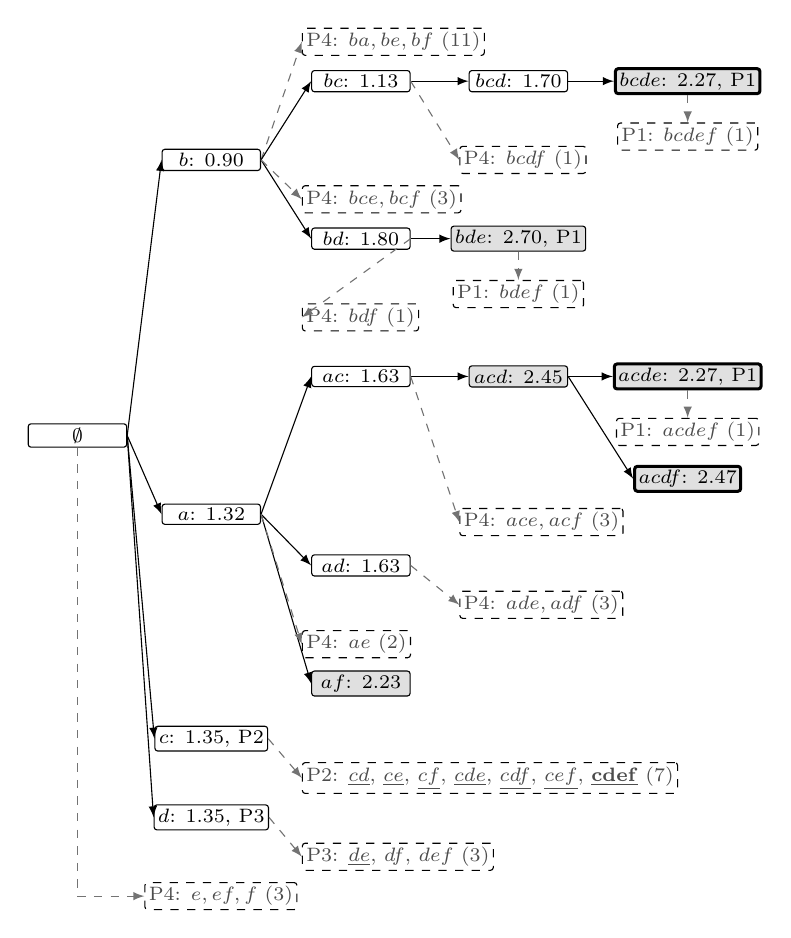
\begin{tikzpicture}[x=1cm, y=0.5cm,
  every node/.style={font=\scriptsize, align=center},
  vis/.style={draw, rounded corners=1pt, inner sep=1.4pt, minimum width=1.25cm},
  hoi/.style={vis, fill=black!12},
  mh/.style={hoi, line width=1.1pt},
  grp/.style={draw, dashed, rounded corners=1pt, inner sep=1.4pt, text=black!70, anchor=west},
  pgrp/.style={draw, dashed, rounded corners=1pt, inner sep=1.4pt, text=black!70, anchor=north},
  ar/.style={-latex}, ard/.style={-latex, dashed, black!55}]
\node[vis] (r)    at (0, -10)    {$\emptyset$};
\node[vis] (b)    at (1.7, -3)   {$b$: 0.90};
\node[grp] (gb)   at (2.85, 0)   {P4: $ba, be, bf$ (11)};
\node[vis] (bc)   at (3.6, -1)   {$bc$: 1.13};
\node[vis] (bcd)  at (5.6, -1)   {$bcd$: 1.70};
\node[mh]  (bcde) at (7.75, -1)  {$bcde$: 2.27, P1};
\node[pgrp](pbcde) at (7.75, -2.05) {P1: $bcdef$ (1)};
\node[grp] (gbcd) at (4.85, -3)  {P4: $bcdf$ (1)};
\node[grp] (gbc)  at (2.85, -4)  {P4: $bce, bcf$ (3)};
\node[vis] (bd)   at (3.6, -5)   {$bd$: 1.80};
\node[hoi] (bde)  at (5.6, -5)   {$bde$: 2.70, P1};
\node[pgrp](pbde) at (5.6, -6.05) {P1: $bdef$ (1)};
\node[grp] (gbd)  at (2.85, -7)  {P4: $bdf$ (1)};
\node[vis] (a)    at (1.7, -12)  {$a$: 1.32};
\node[vis] (ac)   at (3.6, -8.5) {$ac$: 1.63};
\node[hoi] (acd)  at (5.6, -8.5) {$acd$: 2.45};
\node[mh]  (acde) at (7.75, -8.5){$acde$: 2.27, P1};
\node[pgrp](pacde) at (7.75, -9.55){P1: $acdef$ (1)};
\node[mh]  (acdf) at (7.75, -11.1){$acdf$: 2.47};
\node[grp] (gac)  at (4.85, -12.2){P4: $ace, acf$ (3)};
\node[vis] (ad)   at (3.6, -13.3)  {$ad$: 1.63};
\node[grp] (gad)  at (4.85, -14.3) {P4: $ade, adf$ (3)};
\node[grp] (ga)   at (2.85, -15.3) {P4: $ae$ (2)};
\node[hoi] (af)   at (3.6, -16.3)  {$af$: 2.23};
\node[vis] (c)    at (1.7, -17.7){$c$: 1.35, P2};
\node[grp] (gc)   at (2.85, -18.7){P2: \underline{$cd$}, \underline{$ce$}, \underline{$cf$}, \underline{$cde$}, \underline{$cdf$}, \underline{$cef$}, \underline{$\mathbf{cdef}$} (7)};
\node[vis] (d)    at (1.7, -19.7){$d$: 1.35, P3};
\node[grp] (gd)   at (2.85, -20.7){P3: \underline{$de$}, $df$, $def$ (3)};
\node[grp] (gr)   at (0.85, -21.7){P4: $e, ef, f$ (3)};
\draw[ar] (r.east) -- (b.west); \draw[ar] (r.east) -- (a.west); \draw[ar] (r.east) -- (c.west); \draw[ar] (r.east) -- (d.west);
\draw[ard] (r.south) |- (gr.west);
\draw[ard] (b.east) -- (gb.west); \draw[ar] (b.east) -- (bc.west); \draw[ar] (b.east) -- (bd.west); \draw[ard] (b.east) -- (gbc.west);
\draw[ar] (bc.east) -- (bcd.west); \draw[ard] (bc.east) -- (gbcd.west);
\draw[ar] (bcd.east) -- (bcde.west);
\draw[ard] (bcde.south) -- (pbcde.north);
\draw[ar] (bd.east) -- (bde.west); \draw[ard] (bd.east) -- (gbd.west);
\draw[ard] (bde.south) -- (pbde.north);
\draw[ar] (a.east) -- (ac.west); \draw[ar] (a.east) -- (ad.west); \draw[ar] (a.east) -- (af.west); \draw[ard] (a.east) -- (ga.west);
\draw[ar] (ac.east) -- (acd.west); \draw[ard] (ac.east) -- (gac.west);
\draw[ar] (acd.east) -- (acde.west); \draw[ar] (acd.east) -- (acdf.west);
\draw[ard] (acde.south) -- (pacde.north);
\draw[ard] (ad.east) -- (gad.west);
\draw[ard] (c.east) -- (gc.west);
\draw[ard] (d.east) -- (gd.west);
\end{tikzpicture}
\caption{Search of \Algo{} on Table~\ref{tab:example} with $\xi = 2$ (Example~\ref{ex:search}, Table~\ref{tab:trace}). Solid boxes: the 16 visited nodes, with the occupancy of their itemset and the rule (P1, P2, P3) that ends the search below them; items are listed in the search order. Shaded boxes: HOIs; thick boxes: MHOIs. Dashed boxes: the itemsets of the set-enumeration tree that are not visited, grouped by the rule that skips them, with their number; together with the visited nodes they are the 55 itemsets with support at least 2. In the dashed boxes, HOIs are underlined, and the MHOI $cdef$, recorded by rule P2, is in bold.}\label{fig:search}
\end{figure}


\subsection{Correctness}

\begin{theorem}\label{thm:correct}
Algorithm~\ref{alg:main} returns exactly $\MHOI$.
\end{theorem}
\begin{proof}
Every element of $K$ is an HOI: $C$ is added only if $\occ(C) \ge \xi$, and $\cl(C \cup R)$ only if $\occ(C \cup R) \ge \xi$, in which case its closure is an HOI by Lemma~\ref{lem:closure}. Moreover, if \textsc{Mine}$(C)$ returns true, then some HOI contains $C$: this holds when $C$ is an HOI, when P2 applies ($C \subseteq \cl(C \cup R)$), when P3 applies ($C \subseteq C \cup R \subseteq M$), and, by induction on the height of the subtree, when a child $C \cup \{e\} \supsetneq C$ returns true. We show that every MHOI $X$ is in $K$ at the end of the search. The final filter then returns exactly $\MHOI$: every element of $K$ that is not an MHOI is a proper subset of an MHOI, which is in $K$, and an MHOI is not a proper subset of any HOI.

By Lemma~\ref{lem:occsupp}, $\supp(X) \ge \sigma$. Let $x_1 \prec \dots \prec x_t$ be the items of $X$ and $C_i = \{x_1, \dots, x_i\}$; every $C_i$ has support at least $\supp(X) \ge \sigma$, so $C_0 = \emptyset, C_1, \dots, C_t = X$ is a path of the tree. Consider an ancestor $C_i$, $i < t$, with tail $R$. For $j > i$, $\supp(C_i \cup \{x_j\}) \ge \supp(X) \ge \sigma$, so $x_{i+1}, \dots, x_t \in R$, and $X = C_i \cup \{x_{i+1}\} \cup Z'$ with $Z' \subseteq \{x \in R : x \succ x_{i+1}\}$. Since $X$ is an HOI, P1 does not apply at $C_i$, by Theorem~\ref{thm:coupled}, and P4 does not skip $C_{i+1}$, by Corollary~\ref{cor:child}.
If P2 applies at $C_i$, then $X \subseteq C_i \cup R \subseteq \cl(C_i \cup R)$, which is an HOI, so $X = \cl(C_i \cup R)$ by maximality; it is added to $K$ unless it is a subset of an element of $K$, which is an HOI and therefore equals $X$.
If P3 applies at $C_i$, then $X \subseteq C_i \cup R \subseteq M$ for some $M \in K \subseteq \HOI$, so $X = M \in K$.
Hence, unless $X$ has already been placed in $K$, the node holding $X$ is visited. There, every itemset of the subtree is a proper superset of $X$, so none is an HOI. If the tail is empty or P1 applies, $X$ is added to $K$. With a non-empty tail $R$, P2 cannot apply, since $\cl(X \cup R) \supsetneq X$ would be an HOI, and P3 cannot apply, since an element $M \supseteq X \cup R \supsetneq X$ of $K$ would be an HOI. The children are then explored; a child returning true would give an HOI containing a proper superset of $X$, so none does, and $X$ is added to $K$ after the loop.
\end{proof}

\subsection{Complexity}

A node costs one pass over its rows to count the items and to compute $\occ(C)$ and the capacities, and $O(r + c_{\max})$ for P1, where $r$ is the number of rows of the node. Rule P2 intersects the transactions that contain $C \cup R$, and rule P3 compares $C \cup R$ with the recorded itemsets in time linear in their total size. For each child, P4 needs one pass over the rows that contain $e$, and a generated child needs one more pass to build its rows and $O(r \log r)$ to merge them. The final filter compares pairs of recorded itemsets. The number of nodes depends on the data and the threshold; Section~\ref{sec:exp} measures it. The memory consists of the conditional databases on the current path of the search and the recorded itemsets.

%%%%%%%%%%%%%%%%%%%%%%%%%%%%%%%%%%%%%%%%%%%%%%%%%%%%%%%%%%%%%%%%%%%%%%%%%%%%%%%%
\section{Experimental evaluation}\label{sec:exp}

\subsection{Setup}\label{sec:setup}

\paragraph{Methods.}
No algorithm for MHOIs has been published. We compare \Algo{} with the two published HOI miners, each followed by a maximality filter:
\begin{itemize}
\item \textsc{HEP+filter}: HEP \cite{deng2020hoi} computes all HOIs; the HOIs that are subsets of other HOIs are then removed.
\item \textsc{DFHOI+filter}: DFHOI \cite{nguyen2023dfhoi} computes all HOIs, followed by the same filter.
\end{itemize}
The filter sorts the itemsets by decreasing size and keeps an itemset if it is not a subset of an itemset kept before. To reduce the input of the filter, an HOI is not passed to it when an HOI was generated from it during the search (a join parent in HEP, an ancestor in DFHOI); such an HOI has an HOI superset and cannot be maximal. All three methods are therefore exact.

\paragraph{Implementations.}
All methods are written in C. HEP and DFHOI follow the implementations of these algorithms in our pattern-mining code base: the order of the search, the $\ubo$ test of Definition~\ref{def:ubo}, and the shortcut of DFHOI for databases in which all transactions have the same length $L$ (it then computes $\occ(X) = |X| \supp(X) / L$ directly and uses $\supp(X)$ as the bound) are unchanged; items are ordered by increasing support for HEP as in \cite[Section~3.2.3]{deng2020hoi}; the early termination of the $\ubo$ scan described there is not implemented, which affects the time of a $\ubo$ evaluation but not the pruning; and the itemsets are recorded for the filter. \Algo{} and the two baselines use the same input reader, the same comparison tolerance for thresholds and the same final filter. We compare the search effort by the number of \emph{evaluated itemsets}. For HEP and DFHOI, it is the number of itemsets whose list of supporting transactions is computed. For \Algo{}, it is the number of visited nodes (calls of \textsc{Mine} in Algorithm~\ref{alg:main}) plus the number of extensions skipped by rule P4, since computing the child bound $B_e$ requires a pass over the cover of $C \cup \{e\}$; it exceeds the number of visited nodes by a factor between 2.2 and 33 in our experiments.

\paragraph{Platform.}
All experiments ran on one workstation: an Intel Core i7-10700 processor (8 cores, 16 hardware threads, base frequency 2.9~GHz, maximum turbo frequency 4.8~GHz; 32~KiB L1 data cache and 256~KiB L2 cache per core, 16~MiB shared L3 cache) on an ASUS ROG STRIX B460-H GAMING motherboard, with 32~GiB of DDR4 memory and an NVMe solid-state drive, running Ubuntu 24.04.5 LTS with Linux kernel 6.8.0-146-generic. CPU frequency was managed by the \texttt{intel\_pstate} driver with the \texttt{powersave} governor and turbo enabled, which are the default settings of the system. The programs were compiled with GCC 13.3.0 at optimization level \texttt{-O2} (glibc 2.39).

\paragraph{Protocol.}
Every run used one thread and was pinned to one core with \texttt{taskset}. Runtime is the time spent in mining and in the final filter, measured with a monotonic clock; reading the input and building the initial database representation (the root database for \Algo{}, the lists of supporting transactions of single items for HEP and DFHOI) are excluded. Peak memory is the peak resident set size of the process (\texttt{VmHWM} in \texttt{/proc/self/status} \cite{linuxproc}), which includes the loaded database; it is reported in MiB. Each run was limited to 600~s of wall-clock time and 20~GiB of address space. A configuration was repeated five times if its first run took less than 1~s, three times if it took less than 60~s, and once otherwise; we report the median runtime. Runs longer than 60~s are therefore single measurements. For each dataset the thresholds were run from the largest to the smallest, and a method that exceeded a limit was not run at smaller thresholds, since a smaller $\xi$ can only enlarge its search. Visited nodes and outputs did not vary between repetitions.

\subsection{Datasets and thresholds}\label{sec:datasets}

We use the datasets and threshold ranges of Deng \cite[Section~4]{deng2020hoi} (Table~\ref{tab:datasets}): \texttt{mushroom}, derived from the UCI Mushroom data \cite{uci1981mushroom}; \texttt{retail}, market baskets of a Belgian supermarket \cite{brijs1999retail}; \texttt{accidents}, traffic accident records \cite{geurts2003accidents}; \texttt{kosarak}, anonymized click-stream data of a Hungarian online news portal, provided by Ferenc Bodon to the FIMI repository \cite{fimirepository}; and \texttt{T10I4D100K}, a synthetic dataset generated with the IBM generator \cite{agrawal1994fast}. Deng also used \texttt{T40I10D100K}; it is not part of the dataset collection we used, and we did not include it. The files were obtained from the SPMF library \cite{spmfdatasets,fournier2016spmf}; its version of \texttt{mushroom} has 8,416 transactions, whereas the FIMI version used by Deng has 8,124, and its longest \texttt{kosarak} transaction has 2,497 distinct items, against 2,498 in \cite[Table~2]{deng2020hoi}. As in \cite{deng2020hoi}, $\xi$ is given as a percentage of the number of transactions. For each dataset we use five thresholds spanning the range of Table~3 of \cite{deng2020hoi}: 12\% to 4\% for \texttt{mushroom}, 0.05\% to 0.01\% for \texttt{retail}, 30\% to 10\% for \texttt{accidents}, 1\% to 0.2\% for \texttt{kosarak} and 0.1\% to 0.02\% for \texttt{T10I4D100K}. All transactions of \texttt{mushroom} have the same length, so Proposition~\ref{prop:ubo-uniform} applies to it.

\begin{table}[t]
\caption{Datasets. Length: minimum--maximum transaction length (a single value means that all transactions have the same length).}\label{tab:datasets}
\centering
\footnotesize
\begin{tabular}{@{}llrrrr@{}}
\toprule
Dataset & Type & Transactions & Items & Avg.\ length & Length \\
\midrule
\inputrows{tables/datasets.tex}
\botrule
\end{tabular}
\end{table}

\subsection{Correctness}\label{sec:correct-exp}

We verified the implementations against an exact oracle. For \NumOracleDatabases{} random databases with 4 to 10 frequent items and 4 to 24 transactions, of which one third have equal transaction lengths and one third contain additional items that occur once and only lengthen transactions, and for nine thresholds per database ($\xi$ from 5\% to 90\% of the number of transactions, and $\xi = 1.5$), the oracle enumerates every itemset contained in some transaction, computes its occupancy in rational arithmetic and returns the maximal HOIs. In all \NumOracleCases{} cases, \Algo{}, \textsc{HEP+filter}, \textsc{DFHOI+filter} and the six variants of Section~\ref{sec:ablation} returned exactly the oracle's family of itemsets. On the benchmark datasets, all methods that completed a configuration returned the same family of MHOIs. We compared the sorted families: the closed version of the algorithm (Section~\ref{sec:ablation}) returned the same family as HEP and DFHOI in all \SetParityChecked{} configurations completed by at least two of these methods, and \Algo{} returned the same family as the closed version in all \NumSettings{} configurations.

\subsection{Results}\label{sec:results}

Table~\ref{tab:results} reports, for every dataset and threshold, the number of MHOIs, the number of HOIs (from HEP or DFHOI), and the evaluated itemsets, runtime and peak memory of the three methods; Fig.~\ref{fig:counts} and Fig.~\ref{fig:results} plot these measurements.

\paragraph{Number of HOIs and MHOIs.}
Fig.~\ref{fig:counts} compares the number of HOIs with the number of MHOIs. On \texttt{mushroom}, the HOIs outnumber the MHOIs by a factor between \MinHoiMhoiMushroom{} and \MaxHoiMhoiMushroom{}; at $\xi = 4\%$ there are 335,388 HOIs and 107 MHOIs. On \texttt{T10I4D100K} the factor is between \MinHoiMhoiTten{} and \MaxHoiMhoiTten{}, on \texttt{kosarak} between \MinHoiMhoiKosarak{} and \MaxHoiMhoiKosarak{}, and on \texttt{retail} between \MinHoiMhoiRetail{} and \MaxHoiMhoiRetail{}. The factor is largest on \texttt{mushroom}, the dense dataset in which all transactions have the same length, and smallest on the sparse datasets \texttt{retail} and \texttt{kosarak}. On \texttt{accidents} there are no HOIs at 30\%, 25\% and 20\%; at 15\% and 10\%, where neither HOI miner completed, there are 1 and 212 MHOIs.

\begin{figure}[t]
\centering
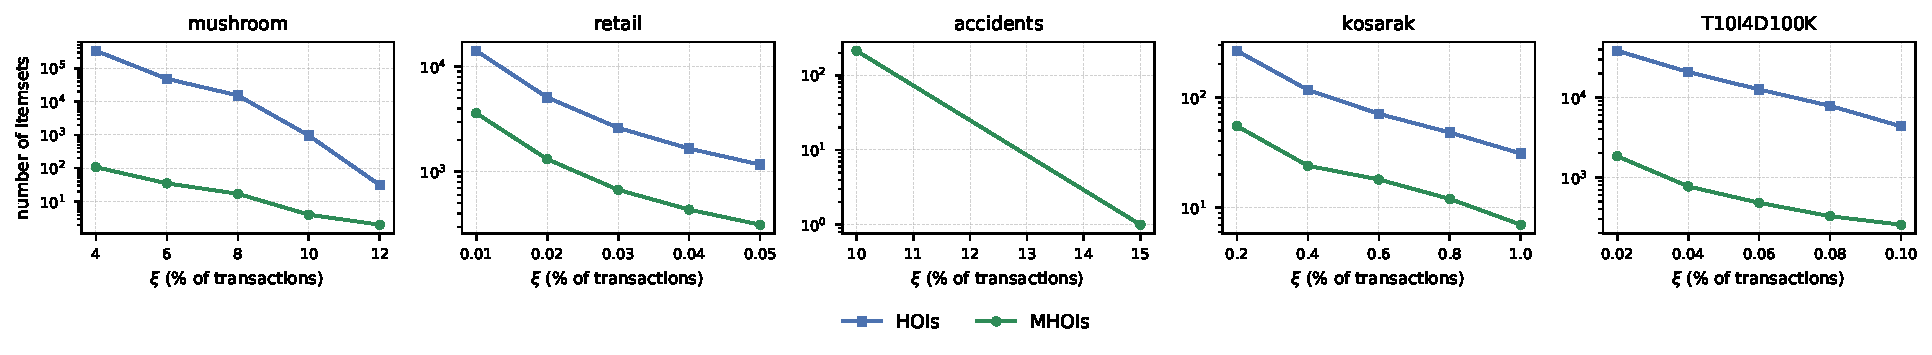
\includegraphics[width=\linewidth]{figures/xi_counts.pdf}
\caption{Number of HOIs (reported by HEP or DFHOI) and of MHOIs as functions of $\xi$. On \texttt{accidents}, there are no HOIs at the thresholds completed by HEP or DFHOI, and only the MHOIs at 15\% and 10\% are shown.}\label{fig:counts}
\end{figure}

\paragraph{Agreement with Deng.}
The numbers of HOIs computed by our implementations of HEP and DFHOI equal those of Table~3 of \cite{deng2020hoi} at every threshold that appears in both studies on \texttt{retail} (1,170, 2,620 and 14,202 at 0.05\%, 0.03\% and 0.01\%), \texttt{kosarak} (31, 71 and 265 at 1\%, 0.6\% and 0.2\%) and \texttt{T10I4D100K} (4,363, 12,640 and 38,588 at 0.1\%, 0.06\% and 0.02\%). On \texttt{mushroom} they do not agree: we find 31, 955, 15,292 and 335,388 HOIs at 12\%, 10\%, 8\% and 4\%, whereas \cite{deng2020hoi} reports 157, 2,723, 15,645 and 331,704. Our version of the dataset differs from Deng's (8,416 against 8,124 transactions), so the counts are not expected to agree, but we have not verified that this difference explains them. On \texttt{accidents}, whose statistics agree with Table~2 of \cite{deng2020hoi} (340,183 transactions, 468 items, average length 33.8, maximum length 51), HEP finds no HOI at 30\%, and DFHOI finds none at 30\%, 25\% and 20\%, whereas \cite{deng2020hoi} reports 15 at 20\%. The absence of HOIs at 20\% can also be checked directly: at 15\% the only MHOI is an itemset of 8 items with support 221,467 and occupancy 51,767.3, that is, 15.2\% of the number of transactions; every HOI at 20\% would be an HOI at 15\% and hence a subset of this itemset, and evaluating its 255 non-empty subsets shows that none has a larger occupancy. We could not determine the cause of the difference.

\paragraph{Evaluated itemsets.}
\Algo{} evaluates fewer itemsets than both baselines in every configuration. Over the configurations completed by both methods, the ratio of the itemsets evaluated by \textsc{HEP+filter} to those evaluated by \Algo{} has median \MedianNodeReductionHep{} (range \MinNodeReductionHep{} to \MaxNodeReductionHep{}, \PairCountHep{} configurations), and the ratio for \textsc{DFHOI+filter} has median \MedianNodeReductionDfhoi{} (range \MinNodeReductionDfhoi{} to \MaxNodeReductionDfhoi{}, \PairCountDfhoi{} configurations). The largest ratios occur on \texttt{accidents} at 30\% and 25\%, where \Algo{} evaluates 33 and 58 itemsets; the smallest occur on \texttt{kosarak}, where the baselines themselves evaluate few itemsets. On \texttt{mushroom}, whose transactions all have length 23, $\ubo$ equals the support (Proposition~\ref{prop:ubo-uniform}), so HEP and DFHOI prune only by support, whereas the bound of Theorem~\ref{thm:coupled} still prunes.

\paragraph{Runtime.}
\Algo{} is faster than \textsc{HEP+filter} in \FasterCountHep{} of \PairCountHep{} configurations and faster than \textsc{DFHOI+filter} in \FasterCountDfhoi{} of \PairCountDfhoi{}; the median runtime ratios (baseline over \Algo{}) are \MedianTimeRatioHep{} and \MedianTimeRatioDfhoi{}. It is slower on \texttt{kosarak}: than \textsc{HEP+filter} at all five thresholds and than \textsc{DFHOI+filter} at the four largest ones, by a factor of up to \MaxSlowdownHep{} and \MaxSlowdownDfhoi{}, respectively. On this dataset the baselines evaluate at most a few thousand itemsets at the larger thresholds, and the cost of a node of \Algo{}, which computes the child bounds and builds a merged conditional database for each child, outweighs the reduction in the number of evaluated itemsets. The reduction in evaluated itemsets is not matched by a reduction in runtime of the same size on the other datasets either, for the same reason. If the time to read the input and build the initial representation is included, which is larger for \Algo{} because it projects and merges the transactions, the counts are unchanged (\FasterEtoECountHep{} of \PairCountHep{} and \FasterEtoECountDfhoi{} of \PairCountDfhoi{}), the median ratios are \MedianEtoERatioHep{} and \MedianEtoERatioDfhoi{}, and the slowdown on \texttt{kosarak} reaches \MaxEtoESlowdownHep{} and \MaxEtoESlowdownDfhoi{}.

\paragraph{Limits.}
\Algo{} completed all \NumSettings{} configurations; its longest run took 7.5~s (\texttt{accidents} at 10\%). On \texttt{accidents}, \textsc{HEP+filter} used 17.1~GiB at 30\% and exceeded the 20~GiB limit at 25\%, because HEP keeps all candidates of a level with their lists of supporting transactions; \textsc{DFHOI+filter} took 525~s at 20\% and exceeded the 600~s limit at 15\%. At 10\%, only \Algo{} completed; it returned 212 MHOIs.

\paragraph{Memory.}
On \texttt{mushroom} and \texttt{accidents}, the peak memory of \textsc{HEP+filter} is much larger than that of the other methods. In most configurations, \Algo{} uses more memory than \textsc{DFHOI+filter}, up to 137~MiB against 88~MiB on \texttt{kosarak}: it stores the conditional databases of the current search path, whereas DFHOI stores lists of transaction identifiers. Over the configurations completed by both methods, the median ratio of the peak memory of \textsc{DFHOI+filter} to that of \Algo{} is \MedianMemRatioDfhoi{}.

\begin{table}[t]
\caption{Results. $\xi$ in \% of the number of transactions; HOIs: number of HOIs reported by HEP or DFHOI; M: \Algo{}, H: \textsc{HEP+filter}, D: \textsc{DFHOI+filter}. TL: time limit (600~s) exceeded; ML: memory limit (20~GiB) exceeded; --: not run because the method failed at a larger threshold.}\label{tab:results}
\centering
\scriptsize
\setlength{\tabcolsep}{2.2pt}
\begin{tabular}{@{}rrrrrrrrrrrr@{}}
\toprule
 & & & \multicolumn{3}{c}{Evaluated itemsets} & \multicolumn{3}{c}{Runtime (s)} & \multicolumn{3}{c}{Peak memory (MiB)} \\
\cmidrule(lr){4-6}\cmidrule(lr){7-9}\cmidrule(l){10-12}
$\xi$ & MHOIs & HOIs & M & H & D & M & H & D & M & H & D \\
\midrule
\inputrows{tables/results.tex}
\botrule
\end{tabular}
\end{table}

\begin{figure}[t]
\centering
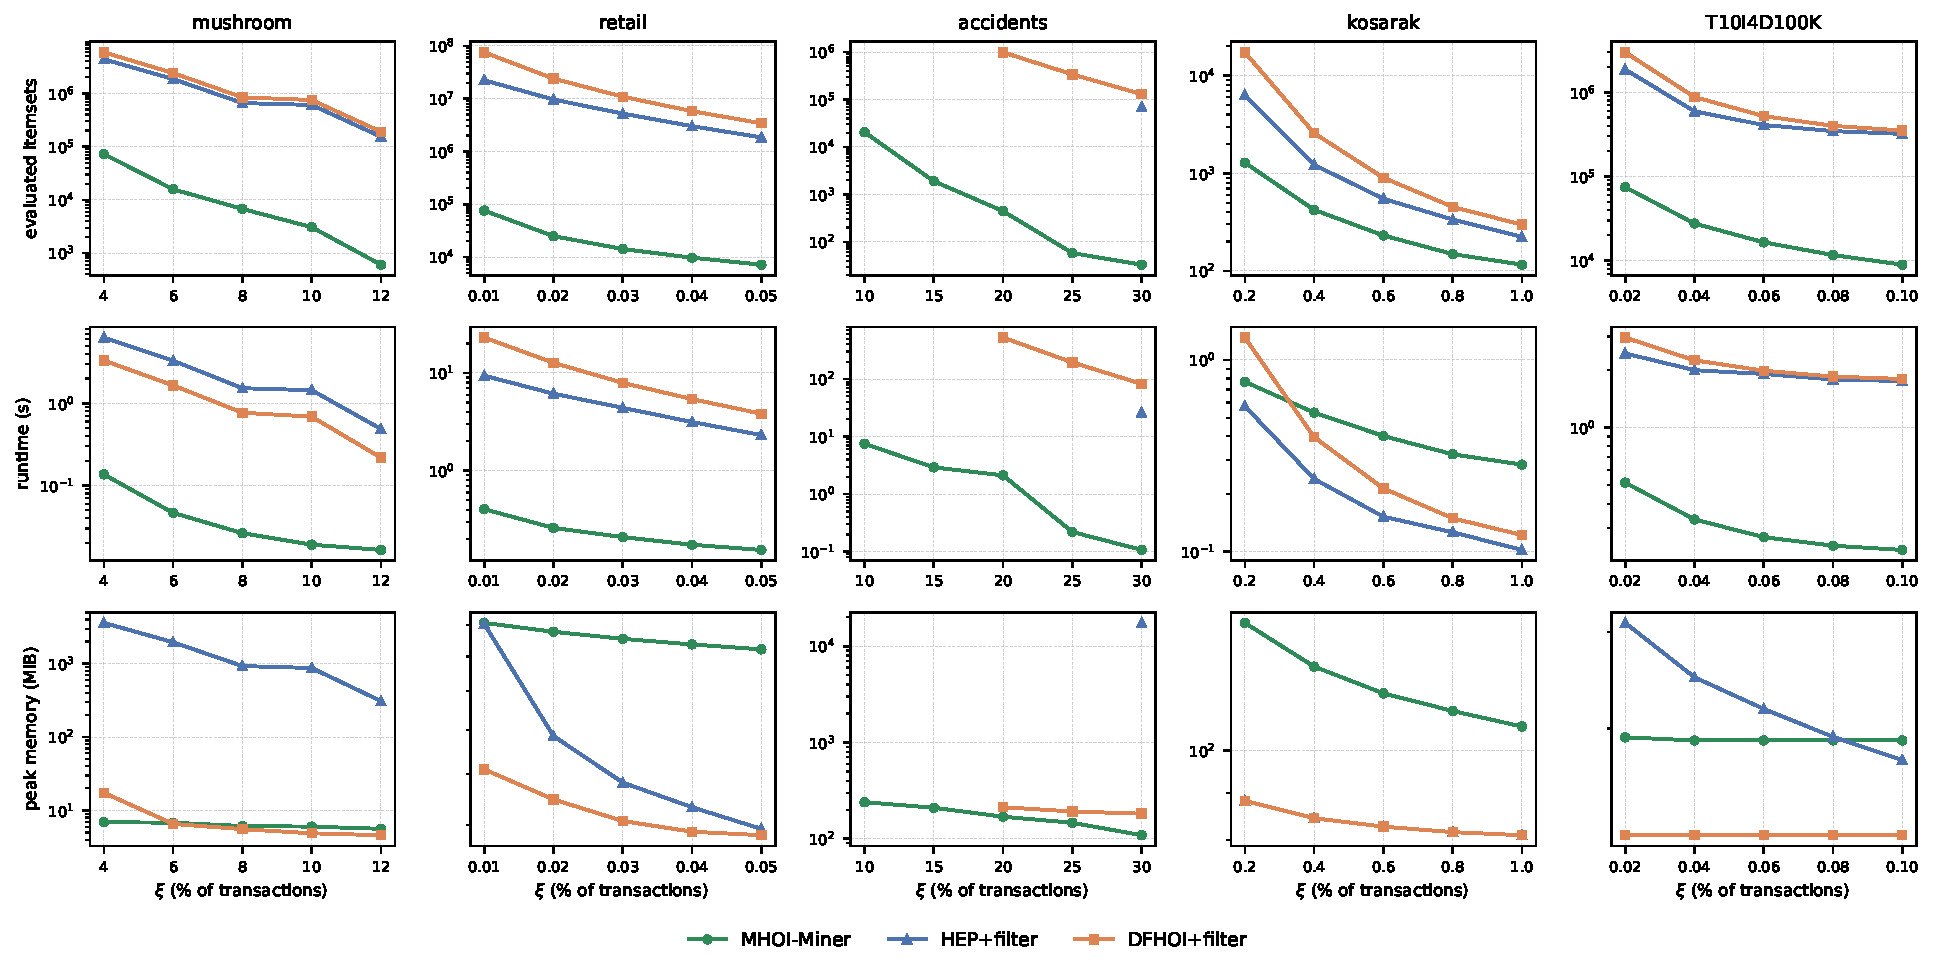
\includegraphics[width=\linewidth]{figures/xi_results.pdf}
\caption{Evaluated itemsets (top), runtime (middle) and peak memory (bottom) as functions of the occupancy threshold $\xi$. Missing points: the method exceeded a limit (Table~\ref{tab:results}).}\label{fig:results}
\end{figure}

\subsection{Ablation}\label{sec:ablation}

Table~\ref{tab:ablation} reports, at the middle threshold of each dataset, the visited nodes and the runtime of \Algo{} and of six variants, measured with the protocol of Section~\ref{sec:setup}. In the variants \emph{no P4}, \emph{$W$} and \emph{$\ubo$}, rule P4 is disabled and rule P1 uses the bound $B$, the per-transaction bound $W$ of Theorem~\ref{thm:pertrans} and the bound $\ubo$ of Definition~\ref{def:ubo}, respectively, so that these three variants differ only in the bound. In \emph{no P2} and \emph{no P3} one rule is disabled. \emph{Closed} enumerates only closed itemsets, by prefix-preserving closure extension \cite{uno2004lcm}, with the same rules; it is the version of the algorithm that we first designed, motivated by Theorem~\ref{thm:maxclosed}.

\begin{itemize}
\item \emph{Bounds.} Without P4, replacing $B$ by $W$ multiplies the number of visited nodes by a factor between \AblNodesWOverB{}, and replacing it by $\ubo$ by a factor between \AblNodesUboOverB{}; the largest factors occur on \texttt{accidents}. With $\ubo$ the runtime grows by a factor of 10 on \texttt{mushroom} and 2.1 on \texttt{accidents}, and by at most 21\% on the other datasets; with $W$ it changes by at most 12\%, the largest increase being on \texttt{accidents}.
\item \emph{Child bound.} Disabling P4 multiplies the runtime by \AblTimeNoPreMin{} to \AblTimeNoPreMax{}. The itemsets that P4 rejects are the children at which P1 would apply, so P4 does not change the number of evaluated itemsets; it avoids building their conditional databases.
\item \emph{Look-ahead and subsumption.} Disabling P2 increases the number of nodes by up to a factor of \AblNodesNoHutMax{} (\texttt{T10I4D100K}) and changes the runtime by at most 4\%; disabling P3 changes the number of nodes by at most 1\% and the runtime by at most 2\%.
\item \emph{Closed itemsets.} The closed version visits between \AblNodesClosedMin{} and \AblNodesClosedMax{} times as many nodes as \Algo{}, fewest on \texttt{mushroom}, but takes between \AblTimeClosedMin{} and \AblTimeClosedMax{} times its runtime: computing closures and testing prefix preservation at every node costs more than it saves on these datasets.
\end{itemize}

\begin{table}[t]
\caption{Ablation at the middle threshold of each dataset ($\xi$ in \%): visited nodes (first line) and runtime (second line). no P4, $W$, $\ubo$: rule P4 disabled and rule P1 with the bound $B$, $W$ or $\ubo$; no P2, no P3: rule disabled; closed: enumeration of closed itemsets only.}\label{tab:ablation}
\centering
\scriptsize
\setlength{\tabcolsep}{2.4pt}
\begin{tabular}{@{}lrrrrrrrr@{}}
\toprule
Dataset & $\xi$ & \Algo{} & no P4 & $W$ & $\ubo$ & no P2 & no P3 & closed \\
\midrule
\inputrows{tables/ablation.tex}
\botrule
\end{tabular}
\end{table}

%%%%%%%%%%%%%%%%%%%%%%%%%%%%%%%%%%%%%%%%%%%%%%%%%%%%%%%%%%%%%%%%%%%%%%%%%%%%%%%%
\section{Case study: retail baskets}\label{sec:case}

To compare MHOIs with maximal frequent itemsets on real data, we use the Online Retail dataset \cite{chen2015onlineretail,chen2012rfm}, which contains the transactions of a United Kingdom non-store online retailer of gifts between 1 December 2010 and 9 December 2011; many of its customers are wholesalers. We grouped the lines of each invoice into one transaction of distinct product codes, after removing cancelled invoices, lines with a non-positive quantity and non-product codes such as postage and manual adjustments; the script is part of the code. The resulting database has \CsTransactions{} transactions and \CsItems{} products; transactions have a median length of \CsMedLen{}, a mean of \CsAvgLen{} and a maximum of \CsMaxLen{}.

With $\xi = \CsXiRel{}$ of the transactions ($\xi = \CsXiAbs{}$), there are \CsNumHOI{} HOIs and \CsNumMHOI{} MHOIs; the support threshold of Lemma~\ref{lem:occsupp} is $\sigma = \CsSigma{}$, at which there are \CsNumMFI{} MFIs. None of the MFIs is an HOI and none of the MHOIs is an MFI, so keeping the MFIs that are HOIs (Theorem~\ref{thm:mfi}) returns nothing here. The two families describe different itemsets. The median MFI has \CsMFIMedSize{} products, support \CsMFIMedSupp{} and occupancy \CsMFIMedOcc{}; it lies in large orders (median length \CsMFIMedLen{} of its supporting invoices), where it covers a small fraction of each. The median MHOI has \CsMHOIMedSize{} product, support \CsMHOIMedSupp{} and occupancy \CsMHOIMedOcc{}, and its supporting invoices have a median length of \CsMHOIMedLen{}.

Of the MHOIs, \CsMHOISingle{} are single products and \CsMHOIMulti{} have two or more (at most \CsMHOIMaxSize{}). Table~\ref{tab:case} lists all MHOIs with two or more products and, for comparison, the single-product MHOIs with the highest occupancy and the MFIs with the highest support. That most MHOIs are single products is a property of occupancy as defined by Deng rather than of the algorithm: occupancy grows with support, so at this threshold the itemsets that reach it are mainly products that appear in many invoices, together with a few sets of products that are bought together often enough. All multi-product MHOIs in Table~\ref{tab:case} consist of variants of one product line (jumbo bags, alarm clocks, hanging-heart T-light holders, Regency teacups with the matching cake stand, picture frames, paper chain kits).

\begin{table}[t]
\caption{Online Retail, $\xi = \CsXiRel{}$ of the transactions. Size: number of products; Support: number of invoices; Length: median number of distinct products of these invoices; occ: occupancy (Definition~\ref{def:occ}).}\label{tab:case}
\centering
\footnotesize
\begin{tabularx}{\linewidth}{@{}Xrrrr@{}}
\toprule
Products & Size & Support & Length & occ \\
\midrule
\inputrows{../case_study/case_study_table.tex}
\botrule
\end{tabularx}
\end{table}

%%%%%%%%%%%%%%%%%%%%%%%%%%%%%%%%%%%%%%%%%%%%%%%%%%%%%%%%%%%%%%%%%%%%%%%%%%%%%%%%
\section{Limitations}\label{sec:limits}

\begin{itemize}
\item MHOIs are not a lossless representation of HOIs: since occupancy is not anti-monotone, the HOIs cannot be recovered from the MHOIs without evaluating the occupancy of their subsets.
\item The measure is the occupancy of Deng, which grows with support. In the case study most MHOIs are single products with high support. Users who want itemsets that cover a large fraction of each supporting transaction regardless of support may prefer the two-threshold formulation of Tang et al.\ \cite{tang2012occupancy}, which this paper does not address.
\item Enumerating only closed itemsets, which Theorem~\ref{thm:maxclosed} suggests, did not pay off in our implementation (Section~\ref{sec:ablation}); a cheaper closure computation might change this. \Algo{} spends more time per node than HEP and DFHOI. It was slower on \texttt{kosarak}, where these algorithms enumerate few itemsets, and it used more memory than DFHOI on the sparse datasets.
\item The comparison uses our C implementations of HEP and DFHOI, not the authors' code; their HOI counts agree with those published by Deng on three of the datasets. We used five of the six datasets of Deng, the SPMF version of \texttt{mushroom}, and one machine. Runtimes depend on the implementations and the machine; visited nodes do not depend on the machine.
\item Subsumption checks (rule P3 and the final filter) scan the recorded itemsets linearly. This was not a bottleneck in our experiments, where at most a few thousand itemsets were recorded, but it would be with many more MHOIs.
\end{itemize}

\section{Conclusion}\label{sec:concl}

We studied the maximal high occupancy itemsets, for the occupancy measure of Deng. Every MHOI is a frequent closed itemset at the support threshold $\lceil \xi \rceil$; maximal frequent itemsets that are HOIs are MHOIs, but MHOIs need not be maximal frequent itemsets, also when all transactions have the same length, so they cannot be obtained by filtering maximal frequent itemsets. When all transactions have the same length, the bound $\ubo$ of Deng reduces to the support. We proposed a bound that fixes the size of a descendant across its supporting transactions, proved that it never exceeds $\ubo$ nor a per-transaction bound, and used it in \Algo{}, a depth-first search of the frequent itemsets with a child bound, head-union-tail look-ahead and subsumption, which we proved correct and verified against an exact oracle. On the datasets and thresholds of Deng, \Algo{} evaluated a median of \MedianNodeReductionHep{} and \MedianNodeReductionDfhoi{} times fewer itemsets than HEP and DFHOI followed by maximality filtering, was faster in most configurations, was the only method that completed all of them, and was slower on \texttt{kosarak}. Reducing the cost per node, for example by avoiding the construction of conditional databases for children that are subsumed, and indexing the recorded itemsets for the subsumption checks, are directions for further work.

\backmatter

\bmhead{Acknowledgements}
Not applicable.

\section*{Declarations}

\begin{itemize}
\item \textbf{Funding:} Funding not applicable. This research received no specific grant from any funding agency in the public, commercial, or not-for-profit sectors.
\item \textbf{Competing interests:} The author declares no competing interests.
\item \textbf{Ethics approval and consent to participate:} Not applicable.
\item \textbf{Consent for publication:} Not applicable.
\item \textbf{Data availability:} The benchmark datasets are publicly available from the SPMF library \cite{spmfdatasets,fournier2016spmf}; \texttt{retail}, \texttt{accidents}, \texttt{kosarak} and \texttt{T10I4D100K} are also distributed by the FIMI repository \cite{goethals2004fimi,fimirepository}. The Online Retail dataset is available from the UCI Machine Learning Repository \cite{chen2015onlineretail} under the CC BY 4.0 licence.
\item \textbf{Materials availability:} Not applicable.
\item \textbf{Code availability:} The source code of all methods and the scripts that reproduce every experiment are available from the author on reasonable request.
\item \textbf{Author contribution:} Q.~Van conceived the method, proved the results, implemented the algorithms, performed the experiments and wrote the manuscript.
\end{itemize}

\bibliography{mfhoi}

\end{document}
